% ===== preamble =====
\usepackage[T1]{fontenc}
\usepackage{lmodern}
\usepackage[margin=1in]{geometry}
\usepackage{amsmath,amssymb,amsthm,mathtools}
\usepackage{enumitem}
\usepackage{microtype}
\usepackage{xcolor}
\usepackage{booktabs}
\usepackage{array}
\usepackage{tikz}
\usetikzlibrary{positioning,calc,arrows.meta,shapes.geometric,fit,backgrounds,patterns}
\usepackage{pgfplots}
\pgfplotsset{compat=1.18}
\usepackage[most]{tcolorbox}
\usepackage[hidelinks]{hyperref}

% ---- theorem environments (shared per-section counter) ----
\theoremstyle{definition}
\newtheorem{definition}{Definition}[section]
\newtheorem{example}[definition]{Example}
\theoremstyle{plain}
\newtheorem{theorem}[definition]{Theorem}
\newtheorem{corollary}[definition]{Corollary}
\newtheorem{proposition}[definition]{Proposition}
\theoremstyle{remark}
\newtheorem*{remark}{Remark}

% ---- exercise list ----
\newlist{exer}{enumerate}{1}
\setlist[exer]{label=\textbf{\thesection.\arabic*},leftmargin=*,itemsep=4pt}

% ---- math shortcuts ----
\newcommand{\R}{\mathbb{R}}\newcommand{\Z}{\mathbb{Z}}\newcommand{\N}{\mathbb{N}}
\newcommand{\comp}[1]{#1^{\mathsf{c}}}
\newcommand{\given}{\mid}
\newcommand{\E}{\mathbb{E}}
\newcommand{\PP}{\mathbb{P}}
\DeclareMathOperator{\Var}{Var}
\DeclareMathOperator{\SD}{SD}
\DeclareMathOperator{\Cov}{Cov}
\DeclareMathOperator{\Corr}{Corr}
\newcommand{\indep}{\perp\!\!\!\perp}
\newcommand{\ind}{\mathbb{1}}            % indicator
\newcommand{\dd}{\,\mathrm{d}}           % differential
\newcommand{\eqd}{\stackrel{d}{=}}       % equal in distribution
% distribution-name operators (use as  X\sim\Bin(n,p)  etc.)
\DeclareMathOperator{\Bin}{Bin}
\DeclareMathOperator{\Hyper}{Hyper}
\DeclareMathOperator{\Geom}{Geom}
\DeclareMathOperator{\NBin}{NegBin}
\DeclareMathOperator{\Pois}{Poisson}
\DeclareMathOperator{\Unif}{Uniform}
\DeclareMathOperator{\Expo}{Exp}
\DeclareMathOperator{\Gam}{Gamma}
\DeclareMathOperator{\Normal}{N}
% common shorthands
\newcommand{\Range}{\mathcal{R}}         % range / support of a random variable
% ---- estimation-theory shortcuts (carried from Chapter 5) ----
\DeclareMathOperator{\Bias}{Bias}
\DeclareMathOperator{\MSE}{MSE}
\DeclareMathOperator*{\argmax}{arg\,max}
\newcommand{\est}[1]{\widehat{#1}}       % estimator hat, e.g. \est\theta
\newcommand{\lik}{L}                       % likelihood function L(theta)
\newcommand{\loglik}{\ell}                 % log-likelihood ell(theta)
\newcommand{\Fish}{\mathcal{I}}            % Fisher information I(theta)
\newcommand{\xbar}{\overline{X}}           % sample mean
\newcommand{\thbar}{\bar\theta}
% ---- hypothesis-testing shortcuts (carried from Chapter 6) ----
\newcommand{\Hnull}{H_0}                    % null hypothesis
\newcommand{\Halt}{H_1}                     % alternative hypothesis
\newcommand{\pval}{p}                       % p-value (in prose: \pval\text{-value})
\DeclareMathOperator{\powerfn}{power}       % power function
\newcommand{\zobs}{z_{\text{obs}}}          % observed z statistic
\newcommand{\tobs}{t_{\text{obs}}}          % observed t statistic
\newcommand{\critreg}{C}                    % critical (rejection) region
\newcommand{\munaught}{\mu_0}               % hypothesized mean
\newcommand{\pnaught}{p_0}                  % hypothesized proportion
\newcommand{\signaught}{\sigma_0}           % hypothesized standard deviation
% ---- Chapters 7-14: shared inference macros (normal-theory, two-sample, regression, ANOVA, nonparametric) ----
\newcommand{\chisq}{\chi^2}                 % chi-square symbol
\newcommand{\ybar}{\overline{Y}}            % sample mean of Y
\newcommand{\dbar}{\overline{D}}            % sample mean of differences (paired)
\DeclareMathOperator{\Fdist}{F}             % F distribution name, e.g. \Fdist_{m,n}
\newcommand{\fobs}{F_{\text{obs}}}          % observed F statistic
\newcommand{\spool}{s_p}                     % pooled standard deviation
% regression
\newcommand{\bhat}{\widehat\beta}           % estimated regression coefficient
\newcommand{\bzero}{\beta_0}
\newcommand{\bone}{\beta_1}
\newcommand{\Sxx}{S_{xx}}
\newcommand{\Sxy}{S_{xy}}
\newcommand{\Syy}{S_{yy}}
\newcommand{\Rsq}{R^{2}}
\newcommand{\yhat}{\widehat{y}}
% ranks (nonparametrics)
\newcommand{\rank}{\operatorname{rank}}
% NOTE: sums-of-squares / mean-squares operators (SSE, SSR, SST, SSTR, SSB, SSW,
% MSE, MSTR, MSB, MSW, etc.) vary by chapter convention -- section authors declare
% the ones they use with \providecommand at the top of their file.

% ---- presentation helpers ----
\newcommand{\keyword}[1]{\textbf{#1}}
\newcommand{\whichrule}[1]{\par\smallskip\noindent$\blacktriangleright$\ \textbf{Which rule, and why?}\enspace #1\par}
\newcommand{\soln}{\par\smallskip\noindent\textbf{Solution.}\enspace}
\newcommand{\steplabel}[1]{\par\smallskip\noindent\textit{#1}\enspace}
% Decision-guide callout box ("how to recognise which rule to use")
\newtcolorbox{strategy}[1][How to recognise which rule to use]{%
  enhanced,breakable,
  colback=black!3,colframe=black!60,boxrule=0.5pt,sharp corners,
  fonttitle=\bfseries,coltitle=black,colbacktitle=black!10,
  title={#1},attach title to upper,after title={\par\smallskip},
  left=8pt,right=8pt,top=6pt,bottom=7pt,toptitle=3pt,bottomtitle=2pt,
  before skip=8pt,after skip=10pt}

% =====================================================================
%  Reusable diagram styles -- consistent, proven-clean geometry.
%  Density pictures (normal / t / chi-square / F): use a pgfplots axis with
%  dens / shade / axline styles. Schematics: nd / term / lbl node styles.
% =====================================================================
\tikzset{
  ptree2/.style={>=Stealth,grow=right,font=\small,
    level 1/.style={sibling distance=38mm,level distance=24mm},
    level 2/.style={sibling distance=19mm,level distance=30mm}},
  ptree3/.style={>=Stealth,grow=right,font=\small,
    level 1/.style={sibling distance=40mm,level distance=24mm},
    level 2/.style={sibling distance=20mm,level distance=28mm},
    level 3/.style={sibling distance=11mm,level distance=30mm}},
  pe/.style={midway,fill=white,inner sep=2pt},
  nd/.style={font=\footnotesize,inner sep=2pt},
  term/.style={font=\footnotesize,inner sep=3pt,draw=black!55,rounded corners},
  lbl/.style={font=\scriptsize,fill=white,inner sep=1.5pt,midway},
  axline/.style={->,>=Stealth,gray!55},
  dens/.style={very thick,black!80},
  shade/.style={black!14},
}

% ---- wrapping framed "conclusion" box: replaces \[ \boxed{...long prose...} \]
% which cannot line-break and ran off the right margin. Put math fragments in $...$.
\providecommand{\conclbox}[1]{%
  \par\smallskip
  \begingroup\centering
  \setlength{\fboxsep}{6pt}%
  \fbox{\parbox{\dimexpr0.92\linewidth-2\fboxsep-2\fboxrule\relax}{\centering #1\par}}\par
  \endgroup
  \smallskip}

% ---- widen the TOC page-number box so 4-digit page numbers (1000+) do not overflow ----
\makeatletter
\renewcommand{\@pnumwidth}{2.4em}
\renewcommand{\@tocrmarg}{3.0em}
\makeatother

% ---- sanity-check marker: render as a filled black box (was a checkmark) ----
% \ensuremath works in both math and text mode, so every existing \checkmark
% (bare in text, $\checkmark$ in math, or inside display math) prints \blacksquare.
\renewcommand{\checkmark}{\ensuremath{\blacksquare}}

% ---- Ch2: axiom theorem environment (shares the per-section definition counter style) ----
\newtheorem{axiom}{Axiom}

% ---- Ch6: "reject H0" shorthand ----
\newcommand{\reject}{\text{reject }\Hnull}

% ---- Ch2: reusable Venn / set-algebra diagram macros (unified house style) ----
% S label tucked in the far top-right corner; A,B labels centred ABOVE their
% circles (never on the boundary, never adjacent to S); event caption BELOW the
% box; circle boundaries always drawn on top of the shading.
\newcommand{\vennShade}{black!16}
\newcommand{\vennframe}{%
  \draw[thin] (-2.7,-1.85) rectangle (2.7,1.85);
  \node[anchor=north east,inner sep=1.5pt] at (2.64,1.79){$S$};
  \draw[thick] (-0.78,0) circle (1.2);
  \draw[thick] ( 0.78,0) circle (1.2);
  \node at (-0.78,1.52){$A$};
  \node at ( 0.78,1.52){$B$};}
\newcommand{\venncap}[1]{\node[below=2pt,font=\footnotesize] at (0,-1.85){#1};}
\newcommand{\vennInter}{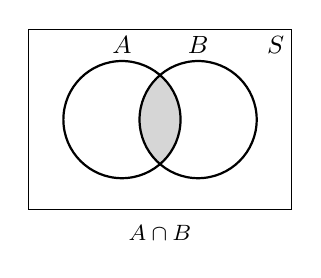
\begin{tikzpicture}[scale=0.62,every node/.style={font=\small}]
  \begin{scope}\clip (-0.78,0) circle (1.2);\fill[\vennShade] (0.78,0) circle (1.2);\end{scope}
  \vennframe\venncap{$A\cap B$}\end{tikzpicture}}
\newcommand{\vennUnion}{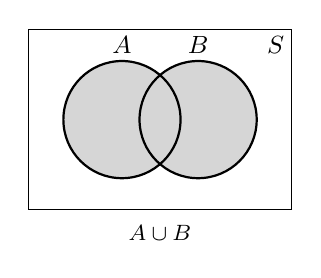
\begin{tikzpicture}[scale=0.62,every node/.style={font=\small}]
  \fill[\vennShade] (-0.78,0) circle (1.2);\fill[\vennShade] (0.78,0) circle (1.2);
  \vennframe\venncap{$A\cup B$}\end{tikzpicture}}
\newcommand{\vennExactlyOne}{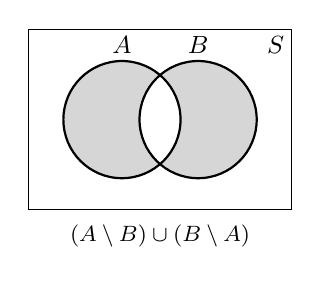
\begin{tikzpicture}[scale=0.62,every node/.style={font=\small}]
  \fill[\vennShade] (-0.78,0) circle (1.2);\fill[\vennShade] (0.78,0) circle (1.2);
  \begin{scope}\clip (-0.78,0) circle (1.2);\fill[white] (0.78,0) circle (1.2);\end{scope}
  \vennframe\venncap{$(A\setminus B)\cup(B\setminus A)$}\end{tikzpicture}}
\newcommand{\vennCompUnion}{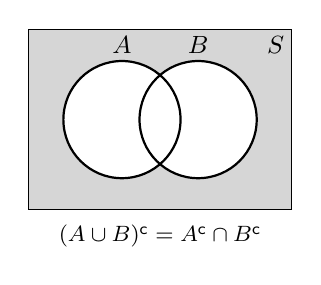
\begin{tikzpicture}[scale=0.62,every node/.style={font=\small}]
  \fill[\vennShade] (-2.7,-1.85) rectangle (2.7,1.85);
  \fill[white] (-0.78,0) circle (1.2);\fill[white] (0.78,0) circle (1.2);
  \vennframe\venncap{$\comp{(A\cup B)}=\comp{A}\cap\comp{B}$}\end{tikzpicture}}
\newcommand{\vennCompInter}{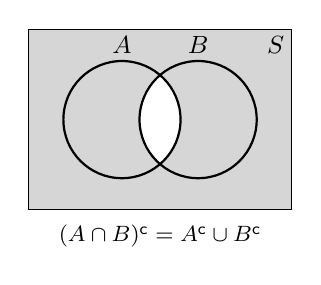
\begin{tikzpicture}[scale=0.62,every node/.style={font=\small}]
  \fill[\vennShade] (-2.7,-1.85) rectangle (2.7,1.85);
  \begin{scope}\clip (-0.78,0) circle (1.2);\fill[white] (0.78,0) circle (1.2);\end{scope}
  \vennframe\venncap{$\comp{(A\cap B)}=\comp{A}\cup\comp{B}$}\end{tikzpicture}}
\newcommand{\vennAminusB}{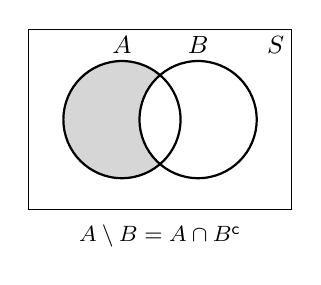
\begin{tikzpicture}[scale=0.62,every node/.style={font=\small}]
  \fill[\vennShade] (-0.78,0) circle (1.2);
  \fill[white] (0.78,0) circle (1.2);
  \vennframe\venncap{$A\setminus B=A\cap\comp{B}$}\end{tikzpicture}}
\newcommand{\vennCompA}{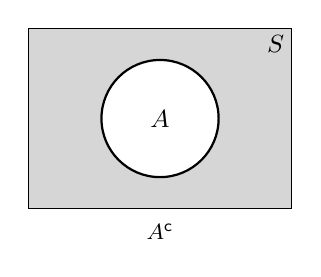
\begin{tikzpicture}[scale=0.62,every node/.style={font=\small}]
  \fill[\vennShade] (-2.7,-1.85) rectangle (2.7,1.85);\fill[white] (0,0) circle (1.2);
  \draw[thin] (-2.7,-1.85) rectangle (2.7,1.85);
  \node[anchor=north east,inner sep=1.5pt] at (2.64,1.79){$S$};
  \draw[thick] (0,0) circle (1.2);\node at (0,0){$A$};
  \venncap{$\comp{A}$}\end{tikzpicture}}
\newcommand{\vennDisjoint}{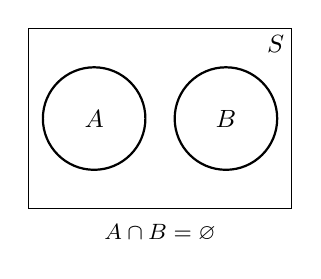
\begin{tikzpicture}[scale=0.62,every node/.style={font=\small}]
  \draw[thin] (-2.7,-1.85) rectangle (2.7,1.85);
  \node[anchor=north east,inner sep=1.5pt] at (2.64,1.79){$S$};
  \draw[thick] (-1.35,0) circle (1.05);\node at (-1.35,0){$A$};
  \draw[thick] ( 1.35,0) circle (1.05);\node at ( 1.35,0){$B$};
  \venncap{$A\cap B=\varnothing$}\end{tikzpicture}}
